\documentclass{book}
	\usepackage[spanish]{babel}
	%\usepackage[utf8]{inputenc}
	\usepackage[latin1]{inputenc}
	\usepackage[total={18cm,21cm},top=2cm, left=2cm]{geometry} %dise�o del documento
	\usepackage{amsmath,amssymb,amsfonts,latexsym,cancel}%paquete de texto matematico
	\usepackage[dvips]{graphicx}
	\usepackage[x11names,table]{xcolor} %paquete de colores en tablas

\begin{document}

\tableofcontents %indice general
\listoftables %indice de tables
\listoffigures %indice de figuras

%% Todas las palabras extranjeras con 
%% itálicas {\it texto en itálicas}

\chapter{Introducci�n}

El presente trabajo muestra el desarrollo de un sistema {\it multi-touch} %% todas las palabras extranjeras
 para crear figuras b�sicas bidimensionales.

%% Esta parte está pendiente de revisar.... no sé que es lo que decidieron al respecto.  --- va seguir existiendo las tags nadamas se simplicaron, el numero de ellas, ya es menor
La interacci�n con el sistema contar� con objetos f�sicos que representan herramientas para dibujar, adem�s se cuenta con otros objetos como herramientas b�sicas para la edici�n del dibujo. \\


El desarrollo del sistema est� enfocado en la integraci�n de tecnolog�as, 
en �ste caso particular se utilizar� la herramienta {\it Kinect}\texttrademark de {\it Microsoft}\textregistered  conectada a una computadora personal, 
adem�s el sistema contar� con reconocimiento de patrones para la selecci�n de herramientas de dibujo o de edici�n del mismo.
%%
\section{Kinect\texttrademark}

{\it Kinect}\texttrademark es un dispositivo que combina una c�mara {\it RGB}, 
un sensor de profundidad y un arreglo de micr�fonos\cite{Robotics}. 
En el Cuadro \ref{tab:1} se listan los elementos principales de {\it Kinect}\texttrademark 
junto con su funci�n.

\begin{table}[h]
\centering
\begin{tabular}{|p{4.8cm}|p{11cm}|}
\hline
{\bf Elemento} & {\bf Funci�n}\\ \hline
Arreglo de micr�fonos& Detecta las voces y las a�sla del ruido ambiental\\ \hline
Proyector de luz infrarroja & Dispara luz infrarroja.\\ \hline
Sensor de profundidad c�mara infrarroja & Detecta la luz que lanza el proyector de luz infrarroja y genera un canal extra al {\it RGB} que trae informaci�n de la profundidad de la escena y es similar a un mapa de disparidad est�reo.\\ \hline
Motor de inclinaci�n & Ajustar hac�a donde est�n dirigidas las c�maras.\\ \hline
Salida de adaptador {\it USB} $2$.$0$ & Conectar un cable para conectar v�a {\it USB} el dispositivo.\\ \hline
C�mara {\it RGB} & Reconocer los tres colores b�sicos. Rojo, verde y azul.\\ \hline
\end{tabular}
\caption{Elementos Principales de {\it Kinect}\texttrademark \cite{ALM}.}
\label{tab:1}
\end{table}

Adem�s cuentan con:
\begin{itemize}
    \item {\it Triple Core PowerPC $970$, $3$.$2$GHz, Hyperthreaded, $2$ threads/core}.
    \item {\it $500$ MHz ATI graphics card}.
    \item {\it $512$ MB RAM}.
\end{itemize}

\section{OpenNI}

Se utiliza {\it OpenNI framework (Open Source Natural Interaction)} versi�n $1$.$3$.$4$.$6$ que es una {\it API} desarrollada por {\it OpenNI organization},  que provee una interfaz para dispositivos que ofrecen una interfaz natural para operar los componentes del {\it middleware}\cite{OpenNI}, en nuestro sistema lo utilizamos para poder comunicar la computadora personal con {\it Kinect}\texttrademark y as� utilizar de la mejor manera para lo que se dise�o el dispositivo {\it Kinect}\texttrademark, que es eliminar los dispositivos f�sicos para controlar, en este caso, la computadora personal.\\

Posee una biblioteca de c�digo abierto para poder trabajar con casi todas las capacidades de {\it Kinect}\texttrademark en {\it Windows}, {\it Linux} y {\it Mac}.

\section{OpenCV}

{\it OpenCV (Open Source Computer Vision Library)} Es una biblioteca {\it GPL}, orientada a la computaci�n visual en tiempo real, utilizada principalmente en el campo de la Interacci�n Computadora - Humano por sus siglas en ingl�s {\it HCI (Human Computer Interaction)} creada y soportada por {\it Intel} desde 1999, y tiene amplia documentaci�n.\\

Actualmente trabajamos con la versi�n $2$.$3$.$1$ de la librer�a {\it OpenCV}.\\

Una de las caracter�sticas m�s importantes de {\it OpenCV} es que las funciones est�n totalmente optimizadas para los procesadores de arquitectura {\it Intel}. Existen versiones para diferentes arquitecturas de procesadores y para diferentes sistemas operativos\cite{Intel}.

\section{Reconocimiento de Patrones}

Para intentar definir que es el Reconocimiento de Patrones (RP) definiremos algunos conceptos\cite{Theodoquidis}.\\

{\bf Reconocimiento:} Proceso de clasificaci�n de un objeto en una o m�s clases.\\

{\bf Objeto:} Es un concepto con el cual representamos los elementos sujetos a estudio. Pueden ser concretos o abstractos.\\

{\bf Patr�n:} Tras los procesos de segmentaci�n, extracci�n de caracter�sticas y descripci�n, cada objeto queda representado por una colecci�n (posiblemente ordenada y estructurada) de descriptores.\\

{\bf Clase:} Es un conjunto de objetos. Al agrupa en clases, se puede hacer de dos formas distintas:
\begin{itemize}
    \item {\it Por pertenencias duras:} Un objeto pertenece o no a una clase.
    \item {\it Por pertenencias difusas:} Los objetos pertenecen parcialmente a una clase. Existen clases con intersecciones no vac�as.
\end{itemize}

Existen varios intentos para definir al reconocimiento de patrones.
\begin{itemize}
    \item La disciplina dedicada a la clasificaci�n de objetos y el pron�stico de fen�menos.\cite{Shulcloper}
    \item Rama del conocimiento, de car�cter multidisciplinario, cuyo objeto de estudio son los procesos de identificaci�n, caracterizaci�n, clasificaci�n y reconstrucci�n sobre conjuntos de objetos o fen�menos, as� como el desarrollo de teor�as, tecnolog�as y metodolog�as relacionadas con dichos procesos.\cite{Shulcloper}
    \item Es la ciencia que se ocupa de los procesos sobre ingenier�a, computaci�n y matem�ticas relacionados con objetos f�sicos y/o abstractos, con el prop�sito de extraer informaci�n que permita establecer propiedades de o entre conjuntos de dichos objetos.\cite{Shulcloper}
\end{itemize}

Con respecto al reconocimiento de patrones, se cuenta con objetos f�sicos los cu�les  hacen la funci�n de botones permitiendo eliminar �stos de la interfaz, �stos objetos tienen asignada una imagen binaria que denominamos {\it tag}(etiqueta), as� la c�mara de {\it Kinect}\texttrademark captura la imagen del escenario, entonces el sistema procesa esa captura donde si se encuentra uno de los objetos f�sicos se decodifica la imagen y se activa la acci�n que se tenga asignada a dicha {\it tag}. Algunas de las {\it tags} tienen m�s de una acci�n que se activan con un giro en cierto �ngulo esto hace que cambie la funci�n que al principio tenia  designada.

\section{Etiquetas (Tag�s)} %% Anteriormente TAG's

Denominamos {\it tag's}(etiquetas) a un conjunto de im�genes binarias en colores blanco y negro que indica el uso de una herramienta.\\

Analizamos tres tipos de im�genes binarias candidatas, las cuales son: {\it reacTIVision fiducials}, C�digo {\it QR} y {\it ARToolKit Marker}.

\subsection{reacTIVision}

Son marcadores especiales (Figura \ref{fig:1.1}) que se desarrollaron en conjunto con el sistema {\it reacTIVision} que es un {\it software} creado especialmente para el rastreo de �stos marcadores que a grandes rasgos son im�genes binarias, espec�ficamente, en blanco y negro.

\begin{figure}[h1]
\centering
\includegraphics[scale=0.4]{ImagenesDocumentacion/reactableTag.ps}
\caption{Ejemplos de marcadores para reacTable.}
\label{fig:1.1}
\end{figure}

Para la identificaci�n de cada marcador se basa en una regi�n grafica adyacente y los rect�ngulos de delimitaci�n. El m�todo combina coincidencias de patrones binarios de gr�ficos topol�gicos (Figura \ref{fig:1.2}) para el reconocimiento y la identificaci�n con simples t�cnicas geom�tricas para calcular la ubicaci�n y orientaci�n de los marcadores\cite{Fiducials}.

\begin{figure}[h1]
\centering
\includegraphics[scale=0.7]{ImagenesDocumentacion/topologiaArbol.ps}
\caption{Algunas simples topolog�as y su correspondiente gr�fico de regi�n adyacente.}
\label{fig:1.2}
\end{figure}
\newpage
Se utilizan algoritmos gen�ticos para la identificaci�n de cada marcador, para m�s detalles consultar\cite{Fiducials}.\\

�stos marcadores est�n disponibles en PDF para su impresi�n as� como el sistema {\it reacTIVision} en la p�gina del proyecto\cite{reacTIVison} y no es necesario producir nuevos marcadores.

\subsection{C�digo QR}

El c�digo de barras de respuesta r�pida por sus siglas en ingl�s {\it QR code*}  ({\it Quick Response Barcode}, Figura \ref{fig:1.3}) es un sistema que permite almacenar informaci�n en un c�digo de barras bidimensional, esto quiere decir que tiene un patr�n de arriba hac�a abajo, de izquierda a derecha, y puede almacenar alrededor de $7,000$ d�gitos (v�ase el Cuadro \ref{tab:2}) mucho m�s que un c�digo de barras convencional, adem�s con la ayuda de una c�mara y un programa especial podemos recuperar la informaci�n de cada c�digo. �ste c�digo esta estandarizado {\it ISO/IEC 18004}.

\begin{figure}[h1]
\centering
\includegraphics[scale=0.5]{ImagenesDocumentacion/codigoQR.ps}
\caption{Ejemplo de C�digo QR.}
\label{fig:1.3}
\end{figure}

\begin{table}[h]
\centering
\begin{tabular}{|c|c|}%{|p{5cm}|p{12cm}|}%
\hline
Num�rico & M�ximo $7,089$ caracteres.\\ \hline
Alfanum�rico & M�ximo $4,296$ caracteres.\\ \hline
Binario & M�ximo $2,953$ caracteres.\\ \hline
Kanji/Kana & M�ximo $1,817$ caracteres.\\ \hline
\end{tabular}
\caption{Capacidad de datos del c�digo QR.}
\label{tab:2}
\end{table}

Existen versiones del c�digo QR desde la $1$ hasta la $40$ y cada una tiene diferentes n�meros de m�dulos (m�dulo se refiere a los puntos blancos y negros que conforman el c�digo QR)\cite{QR}.\\

\hfill{\tiny * QR code es una marca registrada por DENSO WAVE INCORPORATED}\\

Tiene la capacidad de correcci�n de errores (v�ase el Cuadro \ref{tab:3}), si una parte del c�digo est� da�ada, manchada o doblada puede ser interpretado de igual forma.

\begin{table}[h]
\centering
\begin{tabular}{|cc|}%{|p{5cm}|p{5cm}|}%
\hline
\multicolumn{2}{c}{QR Code Error Correction Capability}\\ \hline %\rowcolor{red!20}
Level L & Approx.$7\%$\\ \hline
Level M & Approx.$15\%$\\ \hline
Level Q & Approx.$25\%$\\ \hline
Level H & Approx.$30\%$\\ \hline
\end{tabular}
\caption{Capacidad de correcci�n de errores C�digo QR\cite{QR}.}
\label{tab:3}
\end{table}
\newpage
La decodificaci�n del c�digo {\it QR} puede seguir varios algoritmos a continuaci�n se describe un algoritmo general que puede utilizarse para algunos c�digo de barras  en 2D.

\begin{enumerate}
    \item Binarizaci�n de la imagen.\\
M�todo de Otsu\cite{Otsu}.
    \item Correcci�n de la inclinaci�n.
    \item Correcci�n  geom�trica  de la imagen.
    \item Obtenci�n de los cuatro v�rtices de la imagen.
    \item Obtenci�n de los nuevos valores	 de los v�rtices.
    \item Obtener el valor en cada nuevo pixel.
    \item Normalizaci�n de la imagen.
\end{enumerate}

Existen distintos sistemas que ofrecen la creaci�n de c�digos {\it QR} as� como la decodificaci�n del mismo como {\it ZXing}\cite{ZXing}.

\subsection{ARToolkit}

Son plantillas de forma cuadrada, que se componen de cuadrado negro con un cuadrado blanco cuatro veces m�s peque�o que su centro y un dibujo sencillo en el interior del cuadrado blanco, como se muestra en la  figura \ref{fig:1.4}.

\begin{figure}[h1]
\centering

\includegraphics[scale=1.5]{ImagenesDocumentacion/arToolkit.ps} 
\caption{Ejemplo de ARToolKit Marker.}
\label{fig:1.4}
\end{figure}

Para identificaci�n de la platilla est� basada en la detecci�n de las esquinas con ayuda del algoritmo de {\it fast pose estimation}\cite{ARToolkit}. Los pasos para el tratamiento de estas plantillas son los siguientes:

\begin{enumerate}
    \item La imagen capturada se transforma a una imagen binaria.
    \item Identificamos el marco de color negro.
    \item Extraemos los patrones del dibujo que se encuentra en el interior del marco negro.
    \item Almacenamos los patrones.
    \item Repetimos los primeros tres pasos.
    \item Comparamos los patrones extra�dos con los almacenados.
    \item Aplicamos  funcionalidad de la imagen.
\end{enumerate}

\section{Metodolog�a}

El desarrollo del proyecto se realiz� aplicando el modelo incremental.\cite{Pressman} %% Falta refenrencia al modelo incremental -- no falta ahi abajo esta la referencia del libro Pressman de Ing de SW 
Esta metodolog�a tiene la ventaja de ser din�mica y flexible, adem�s permite usar las salidas de las etapas precedentes, 
como entradas en las etapas sucesivas y facilita corregir cualquier error detectado o llevar a cabo mejoras en 
los distintos productos que se generan a lo largo de su aplicaci�n\cite{Pressman}.\\ 

Esta metodolog�a, se basa en la metodolog�a en cascada. El uso de esta metodolog�a dentro del desarrollo del proyecto proporcion�:
\begin{itemize}
	\item Definici�n de actividades a llevarse a cabo en el tiempo de realizaci�n del Trabajo Terminal.
	\item Unificaci�n de criterios en la organizaci�n para el desarrollo del proyecto.
	\item Puntos de control y revisi�n.
	\item Seguimiento de secuencias ascendentes o descendentes en las etapas del desarrollo.
	\item Cumplimiento de etapas o fases en paralelo, por lo que es m�s flexible que la estructurada.
\end{itemize}

\subsection{Paradigma}

El paradigma ser� Orientado a Objetos, porque la {\it API} usada de {\it OpenCV} est� en lenguaje  {\it C++}, que permite la manipulaci�n de objetos, ya que primero definen objetos, para luego enviarles mensajes solicit�ndoles que realicen sus m�todos por s� mismos.\\

El uso del paradigma proporciona:
\begin{itemize}
    \item No modela la realidad, sino la forma en que las personas comprenden y procesan la realidad.
    \item Es un proceso ascendente basado en una abstracci�n de clases en aumento.
    \item Se basa en identificaci�n de objetos, definici�n y organizaci�n de librer�as de clases, y creaci�n de macros para aplicaciones espec�ficas.
    \item Utiliza menor cantidad de c�digo.
    \item Es reutilizable.
\end{itemize}

\section{Objetivos}
\subsection{Problem�tica}
Ofrecer una alternativa al teclado y mouse con una interfaz de usuario natural donde ya no se interactu� directamente con un dispositivo electr�nico, junto con esto querer desarrollar alg�n sistema que probara que se pod�a utilizar {\it Kinect}\texttrademark junto con la computadora personal.

\subsection{General}%%
Desarrollar un sistema con una interfaz de usuario natural, asistido con la herramienta de entretenimiento {\it Kinect}\texttrademark y reconocimiento de patrones. 

\subsection{Particulares} %%
\begin{itemize}
	\item Lograr una configuraci�n para usar {\it Kinect}\texttrademark con la computadora personal, para desarrollar un sistema.
	\item Implementar una interfaz sin involucrar dispositivos electronicos como una pantalla tactil.
	\item Eliminar uso del {\it mouse} en nuestro sistema.
	\item Eliminar uso del teclado en nuestro sistema.
\end{itemize}
%\item Reconocer una imagen binaria la cual puede ser rotada para diferentes acciones.

\section{Justificaci�n}

Una de las principales caracter�sticas sobre la dificultad del desarrollo de los sistemas {\it multi-touch} basado en tecnolog�a \textquotedblleft reciente\textquotedblright en el caso de {\it Kinect}\texttrademark era la falta de documentaci�n fiable al momento de plantear este proyecto (Octubre - Diciembre 2011) ya que no se contaba con drivers capaces de explotar todas las caracter�sticas de {\it Kinect}\texttrademark ni un entorno de desarrollo estable por parte de {\it MS} o de la comunidad de {\it software} libre. El desarrollo de �ste sistema busca contribuir a la creaci�n de documentaci�n formal que permitir� que futuras generaciones tengan mayor cantidad de fuentes fiables y por lo tanto se interesen por la creaci�n de sistemas basados en movimientos, logrando ser un aportador m�s al crecimiento de dichos entornos.\\

Adem�s, permitir que los alumnos de la Escuela Superior de C�mputo que se encuentren cursando o tengan inter�s en el reconocimiento de patrones o semejantes, trabajen con los actuales dispositivos de captura de imagen, siendo en nuestro caso {\it Kinect}\texttrademark de {\it Microsoft}\textregistered, dejando a un lado su complejidad y crear un mayor inter�s, buscando cambiar el enfoque de dicha herramienta en donde el alumno no la vea como un proyecto de Trabajo Terminal sino como pr�cticas semestrales, lo que brindar� mayor competitividad e integraci�n de nuevas tecnolog�as.\\

Esta integraci�n de tecnolog�as ofrece una alternativa al {\it mouse} y al teclado pudiendo as� evitar enfermedades ya conocidas causadas por �stos dispositivos como lo es el s�ndrome de t�nel carpiano\cite{carpiano}. 

\subsection{Estado del arte}

Actualmente no se cuenta con un sistema de dibujo como el que se pretende realizar, a la fecha de la documentaci�n del estado del arte (Marzo 2012) existen otros trabajos que tambi�n manejan {\it Kinect\texttrademark, OpenCV y OpenNI}, elementos con los que se llevar� acabo el desarrollo de nuestro sistema, de los cuales vamos a mencionar algunos a continuaci�n.\\

Gracias a la aparici�n de {\it drivers} que permiten la interacci�n entre el dispositivo {\it Kinect}\texttrademark, que primeramente era exclusivo para la consola de videojuegos {\it Xbox} $360$ de {\it Microsoft}\textregistered, y la computadora, se comenzaron a realizar aplicaciones que permiten al usuario tener una interacci�n m�s natural, permitiendo ser ellos mismos el control de la aplicaci�n. Deb�do a que era una tecnolog�a \textquotedblleft reciente\textquotedblright exist�a poca documentaci�n formal acerca de proyectos relacionados.

\subsubsection{Hand Tracking - Kinect with OpenCV 2.2 and OpenNI}

Es una aplicaci�n sencilla que en primera instancia reconoce la mano de un usuario, como  un punto permitiendo realizar trazos a mano alzada (Figura \ref{fig:1.5}), la aplicaci�n puede  cambiar el punto con que se realizar el trazo entre una mano y otra juntando las manos para volverlas a separar as� queda realizado el cambio. Esta aplicaci�n tambi�n permite la  identificaci�n del cuerpo (Figura \ref{fig:1.6}) con lo que se toman a ambas manos como puntos de  inter�s, uno de ellos se encarga de realizar el trazo y con el otro se puede seleccionar el color.

\begin{figure}[h1]
\centering
\includegraphics[0cm,0cm][18cm,6cm]{ImagenesDocumentacion/handTracking.ps} %[scale=1.5]
\caption{Hand Tracking.}
\label{fig:1.5}
\end{figure}

La relaci�n que existe entre este trabajo y el que se pens� realizar es que ambos  deben poder generar dibujos identificando un punto de interes con el cual se van a hacer los trazos adem�s de seleccionar el color y agregar otra funcionalidades. �ste sistema no cuenta con una documentaci�n y lo �nico que se puede obtener es lo que se visualiza en un video subido a la red\cite{Tracking}.

\begin{figure}[h1]
\centering
\includegraphics[0cm,0cm][16.5cm,7cm]{ImagenesDocumentacion/reconocimientoCuerpo.ps} %[scale=1.5]
\caption{Reconocimiento del cuerpo.}
\label{fig:1.6}
\end{figure}

\subsubsection{Kinect Active Projection Mapping}

Es una aplicaci�n que trabaja con {\it Kinect\texttrademark, OpenCV y OpenNI}, adem�s comparte la idea de mantener un �rea de trabajo y una proyeci�n, de tal modo el usuario interact�a directamente sobre el �rea designada (Figura \ref{fig:1.7}).\\

En este proyecto se utiliza el kinect para reconocer el cuerpo, la posici�n de las manos principalmente. El sistema crea un efecto visual en  sobre las manos y entre ellas por medio de una imagen que es proyectada sobre una pantalla detras de el usuario\cite{Mapping}.\\

Esta aplicaci�n ha sido desarrollada en el {\it Computer Fusion Laboratory} como parte del programa de ingenieria de la {\it Temple University}. La p�gina donde se dan m�s detalles del proyecto se encuentra a�n en construcci�n. Y por el momento los recursos no est�n disponibles.

\begin{figure}[h1]
\centering
\includegraphics[scale=0.8]{ImagenesDocumentacion/proyeccionManos.ps} %[0cm,0cm][16.5cm,4.5cm]
\caption{Proyecci�n de im�gen sobre un �rea de trabajo.}
\label{fig:1.7}
\end{figure}

\subsubsection{Aldebaran Nao Kinect Controller}

Es un proyecto donde se controla por medio de {\it Kinect}\texttrademark a un robot (Figura \ref{fig:1.8}), organismo aut�nomo programable y de mediana estatura desarrollado por la empresa Francesa {\it Aldebaran Robotics}. Esta aplicaci�n ha sido desarrollada en {\it Technical University Bergakademie Freiberg} en Alemania por Erik Berger y Heni Ben Amor. Existe informaci�n adicional de este proyecto en la p�gina oficial de la universidad \cite{Freiberg}, Pero se encuentra en idioma Alem�n.\\

Este proyecto no tiene mucha relaci�n en cuanto a la funcionalidad del trabajo que se desea realizar, pero se considera por el hecho de tambi�n emplear los elementos que utilizaremos en nuestro sistema. 

\begin{figure}[h1]
\centering
\includegraphics[0cm,0cm][16.5cm,7cm]{ImagenesDocumentacion/interaccionRobot.ps} %[scale=0.8]
\caption{Interacci�n con robot autom�ta programable.}
\label{fig:1.8}
\end{figure}
 %% agrega la extension .tex automaticamente
\chapter{Análisis}

En este capítulo se describe en análisis realizado para la creación del sistema. 
El análisis se presenta según los cuatro módulos que se reconocieron en un principio: 

\begin{enumerate}
 \item Editor Básico de Dibujo
\item Reconocimiento de trazos a mano alzada
\item Proyección sobre el área de trabajo 
\item Implementación de las herramientas físicas para el dibujo.
\end{enumerate}

Con el análisis correspondiente a los módulos tres y cuatro se fijarán las especificaciones necesarias, además se mencionarán todas aquellas problemáticas detectadas en los procesos.  

%% esta parte está fuera de lugar, .....
Se mostrará el estudio de factibilidad correspondiente al proyecto, posteriormente se expondrá el documento de definición de requerimientos, para finalizar con la especificación de requerimientos. 
En el anexo se mostrarán los diagramas generales y de los primeros dos módulos que representan   los procesos mencionados.
 %% agrega la extension .tex automaticamente
\chapter{Dise�o}

\section{Arquitectura del Sistema}

A continuaci�n se muestra la estructura o esqueleto del sistema, para ello se utilizo la abstracci�n de capas \cite{capas},\cite{Layer} el cual cuenta con tres capas, una capa superior, una intermedia y una inferior, las cuales se describen enseguida(Figura \ref{fig:3.1}):

\begin{itemize}
    \item La capa superior: Representa el {\it software} que implementa el sistema, con el que interact�a el usuario.
    \item La capa intermedia: Representa la {\it API (OpenCV)} y el {\it driver (OpenNI)}, para la comunicaci�n entre el hardware y el sistema.
    \item La capa inferior: Muestra los dispositivos ({\it hardware}), que se encargan de la captura y proyecci�n de la imagen.
\end{itemize}

\begin{figure}[h1]
\centering
\includegraphics[scale=0.6]{ImagenesDocumentacion/ArquitecturaCapas.ps} %[0cm,0cm][16.5cm,7cm]
\caption{Arquitectura - abstracci�n de capas.}
\label{fig:3.1}
\end{figure}

\section{Diagramas Generales del Sistema}
En esta secci�n se mostrar�n los diagramas generales, que se llevaron acabo para la realizaci�n del sistema, los cuales son: de casos de uso(Figura \ref{fig:3.2}), de clases(Figura \ref{fig:3.3}), de secuencia(Figura \ref{fig:3.4}) y de estados(Figura \ref{fig:3.5}).
\subsection{Diagrama General de Casos de Uso.}
\begin{figure}[h1]
\centering
\includegraphics[scale=0.8]{ImagenesDocumentacion/generalDCasosU.ps} %[0cm,0cm][16.5cm,7cm]
\caption{Diagrama General de Casos de Uso.}
\label{fig:3.2}
\end{figure}
\newpage
\subsubsection{Especificaci�n de casos de uso}
En este aparto se describen los casos de uso del sistema,donde se explica cada caso de uso correspondiente a su Cuadro, en el cual se tiene su descripci�n,el actor, las condiciones con las que se debe contar,su flujo, asi como anotiaciones y/o excepciones.\\\\
Abreviaturas:\\\\
E.C.U.: Especificaci�n de Caso de Uso\\\\
TT-2011-B007: Trabajo Terminal con No. de Registro 2011-B007\\\\

{\bf Caso de Uso: Inicializar Sistema}
\begin{table}[h]
\centering
\begin{tabular}{|p{5cm}|p{9cm}|}
\hline
Especificaci�n del Caso de Uso: & Inicializar Sistema \\ \hline
ID: & E.C.U-1\\ \hline
Nombre: &  Inicializar el sistema\\ \hline
Descripci�n: & El usuario inicializara la aplicaci�n del sistema\\ \hline
Autor:	& TT-2011-B007\\ \hline
Actores: & Usuarios (M�ximo dos usuarios)\\ \hline
Precondici�n: & Dispositivos conectados (kinect, proyector),Driver y API instalados\\ \hline
Pos Condici�n: & Sistema inicializado con �xito\\ \hline
Flujo Normal de eventos: & Iniciar:\\
& 1.	El actor iniciara el sistema de dibujo en 2D multi-touch con reconocimiento de patrones\\
& 2.	Una vez iniciado, el usuario podr� interactuar con el sistema
\\\hline
Flujos Alternos: & Sistema ya iniciado:\\
& 1.	Si ya se inicio, se proceder� con el paso 2\\ \hline
Excepciones: & Ninguna\\ \hline
Anotaciones: & Ninguna\\ \hline
\end{tabular}
\caption{Inicializar Sistema.}
\label{tab:3.1}
\end{table}

\newpage
{\bf Caso de Uso: Rotar Herramienta}
\begin{table}[h]
\centering
\begin{tabular}{|p{5cm}|p{9cm}|}
\hline
Especificaci�n del Caso de Uso: & Rotar Herramienta\\ \hline
ID: & E.C.U-2\\ \hline
Nombre: &  Rotar Herramienta\\ \hline
Descripci�n: & El usuario rotar� la herramienta llamada TAG, en el �rea de trabajo\\ \hline
Autor: & TT-2011-B007\\ \hline
Actores: & Usuarios (M�ximo dos usuarios)\\ \hline
Precondici�n: & Dispositivo kinect conectado\\ \hline
Pos Condici�n: & La herramienta estar� situada en el �rea de trabajo\\ \hline
Flujo Normal de eventos: & Colocaci�n de la Herramienta:\\
& 1.	El actor  seleccionara la herramienta que desea utilizar\\
& 2.	Se rotar� la herramienta en el �rea de trabajo
\\\hline
Flujos Alternos: & Posici�n de Herramienta:\\
& 1.	Despu�s de rotar la herramienta se acomodara en una posici�n para hacer algo distinto en el editor, si se trata de una herramienta para hacer cambios\\ \hline
Excepciones: & Herramienta mal posicionada:\\
& 1.	Si la herramienta  no est� del lado indicado � de la posici�n correcta, no se podr� trabajar con ella\\ \hline
Anotaciones: & Solo se puede utilizar una herramienta en el �rea a la vez \\ \hline
\end{tabular}
\caption{Rotar Herramienta.}
\label{tab:3.2}
\end{table}

\newpage
{\bf Caso de Uso: Reconocer Herramienta}
\begin{table}[h]
\centering
\begin{tabular}{|p{5cm}|p{9cm}|}
\hline
Especificaci�n del Caso de Uso: & Reconocer Herramienta\\ \hline
ID: & E.C.U-3\\ \hline
Nombre: &  Reconocer Herramienta\\ \hline
Descripci�n: & Cuando ya se encuentre colocada la tag , kinect tomar� video  del escenario el cual ser� procesado por la PC y se detecta  la tag que este ubicada en el �rea de trabajo\\ \hline
Autor: & TT-2011-B007\\ \hline
Actores: & Usuarios (M�ximo dos usuarios)\\ \hline
Precondici�n: & Dispositivo kinect conectado\\ \hline
Pos Condici�n: & Quedar� habilitada la acci�n correspondiente a la tag.\\ \hline
Flujo Normal de eventos: & Detecci�n de imagen:\\
& 1.	Una vez colocada la herramienta en el �rea, el kinect captura video del escenario para procesarla\\
& 2.	Una vez que se procese, se podr� hacer la acci�n que tiene prevista la herramienta\\
& 3.	El actor  podr� seleccionar � dibujar en el �rea de trabajo
\\\hline
Flujos Alternos: & Posici�n de Herramienta:\\
& 1.	Si se trata de una herramienta para hacerle cambios a lo dibujado, entonces se mover� de posici�n la herramienta(giro), para tener dichos cambios, esto solo aplica en escalar y color\\ \hline
Excepciones: & Imagen  incorrecta:\\
& 1.	Si la tag no corresponde con las indicadas en el sistema ,no se podr� reconocer\\ \hline
Anotaciones: & Solo se puede utilizar una herramienta en el �rea a la vez \\ \hline
\end{tabular}
\caption{Reconocer Herramienta.}
\label{tab:3.3}
\end{table}

\newpage
{\bf Caso de Uso: Seleccionar}
\begin{table}[h]
\centering
\begin{tabular}{|p{5cm}|p{9cm}|}
\hline
Especificaci�n del Caso de Uso: & Seleccionar\\ \hline
ID: & E.C.U-4\\ \hline
Nombre: &  Seleccionar\\ \hline
Descripci�n: & Selecci�n del dibujo para poder realizar alg�n cambio sobre �ste.\\ \hline
Autor: & TT-2011-B007\\ \hline
Actores: & Usuarios (M�ximo dos usuarios)\\ \hline
Precondici�n: & Dispositivo kinect conectado, dibujo previo\\ \hline
Pos Condici�n: & Se selecciono con �xito el dibujo.\\ \hline
Flujo Normal de eventos: & Selecci�n:\\
& 1.	Ya que se tenga el dibujo, el actor, seleccionar� la imagen mediante el uso de su dedo\\
& 2.	Para por ultimo poder hacer alg�n cambio en la imagen\\ \hline
Flujos Alternos: & Dibujo seleccionado:\\
& 1.	Una vez que se est� en el paso 1 del flujo normal se puede  cambiar el tipo de acci�n para modificar el dibujo\\ \hline
Excepciones: & Selecci�n de dibujo:\\
& 1.	Trazos a mano alzada no podr�n ser seleccionados.\\ \hline
Anotaciones: & Solo se puede utilizar una herramienta en el �rea a la vez, el usuario solo puede utilizar un dedo de la mano. \\ \hline
\end{tabular}
\caption{Seleccionar.}
\label{tab:3.4}
\end{table}

\newpage
{\bf Caso de Uso: Herramienta Invalida}
\begin{table}[h]
\centering
\begin{tabular}{|p{5cm}|p{9cm}|}
\hline
Especificaci�n del Caso de Uso: & Herramienta Invalida\\ \hline
ID: & E.C.U-5\\ \hline
Nombre: & Herramienta Invalida\\ \hline
Descripci�n: & Si se llega a poner otro objeto que no se tenga considerado como herramienta del sistema, entonces el  sistema no reconocer� dicha herramienta.\\ \hline
Autor: & TT-2011-B007\\ \hline
Actores: & Usuarios (M�ximo dos usuarios)\\ \hline
Precondici�n: & Dispositivo kinect conectado\\ \hline
Pos Condici�n: & El objeto es una herramienta invalida para el sistema.\\ \hline
Flujo Normal de eventos: & Herramienta Err�nea:\\
& 1.	Si el actor llegar� a poner otro objeto que no se considero en el sistema, entonces no se podr� reconocer el objeto\\ \hline
Flujos Alternos: & Verificar Herramienta:\\
& 1.	Si pasara el paso 1 del  evento, entonces se verificar�a  si la herramienta es la correcta o est� colocada correctamente.\\ \hline
Excepciones: & Ninguna\\ \hline
Anotaciones: & Solo se puede utilizar una herramienta en el �rea a la vez.\\ \hline
\end{tabular}
\caption{Herramienta Invalida.}
\label{tab:3.5}
\end{table}

\newpage
{\bf Caso de Uso: Mover}
\begin{table}[h]
\centering
\begin{tabular}{|p{5cm}|p{9cm}|}
\hline
Especificaci�n del Caso de Uso: & Mover\\ \hline
ID: & E.C.U-6\\ \hline
Nombre: & Mover\\ \hline
Descripci�n: & Esta herramienta nos permite mover de posici�n alguna figura, para ello debe estar seleccionada.\\ \hline
Autor: & TT-2011-B007\\ \hline
Actores: & Usuarios (M�ximo dos usuarios)\\ \hline
Precondici�n: & Dispositivo kinect conectado\\ \hline
Pos Condici�n: & Reconocimiento de la herramienta, poder mover con �xito el dibujo.\\ \hline
Flujo Normal de eventos: & Mover:\\
& 1.	El actor seleccionar� el dibujo que desea mover\\
& 2.	El actor proceder� a mover el dibujo seleccionado sobre el �rea.\\ \hline
Flujos Alternos: & Ninguno.\\ \hline
Excepciones: & Selecci�n de dibujo:\\
& 1.	Trazos a mano alzada no podr�n ser seleccionados.\\ \hline
Anotaciones: & Solo se puede utilizar una herramienta en el �rea a la vez , el usuario solo puede utilizar  un dedo de  la mano.\\ \hline
\end{tabular}
\caption{Mover.}
\label{tab:3.6}
\end{table}

\newpage
{\bf Caso de Uso: Cambiar Color}
\begin{table}[h]
\centering
\begin{tabular}{|p{5cm}|p{9cm}|}
\hline
Especificaci�n del Caso de Uso: & Cambiar Color\\ \hline
ID: & E.C.U-7\\ \hline
Nombre: & Cambiar Color\\ \hline 
Descripci�n: & Esta herramienta nos permite cambiar de color alguna figura seleccionada.\\ \hline
Autor: & TT-2011-B007\\ \hline
Actores: & Usuarios (M�ximo dos usuarios)\\ \hline
Precondici�n: & Dispositivo kinect conectado\\ \hline
Pos Condici�n: & Reconocimiento de la herramienta, poder cambiar de color con �xito el dibujo.\\ \hline
Flujo Normal de eventos: & Color:\\
& 1.	El actor mover� las herramientas que se tiene para la gama de colores(64 colores), una por R, otra por G y una de B, para dar dichas combinaciones\\
& 2.	Se rotar� la herramienta hasta conseguir el color deseado en el dibujo.\\
& 3.	El actor dibujara su trazo con el color escogido\\ \hline
Flujos Alternos: & Ninguno.\\ \hline
Excepciones: & Selecci�n de dibujo:\\
& 1.	Trazos a mano alzada no podr�n ser seleccionados.\\ \hline
Anotaciones: & Solo se puede utilizar una herramienta en el �rea a la vez , el usuario solo puede utilizar  un dedo de  la mano.\\ \hline
\end{tabular}
\caption{Cambiar Color.}
\label{tab:3.7}
\end{table}

\newpage
{\bf Caso de Uso: Escalar}
\begin{table}[h]
\centering
\begin{tabular}{|p{5cm}|p{9cm}|}
\hline
Especificaci�n del Caso de Uso: & Escalar\\ \hline
ID: & E.C.U-8\\ \hline
Nombre: & Escalar\\ \hline 
Descripci�n: & Esta herramienta nos permite cambiar de tama�o alguna figura seleccionada.\\ \hline
Autor: & TT-2011-B007\\ \hline
Actores: & Usuarios (M�ximo dos usuarios)\\ \hline
Precondici�n: & Dispositivo kinect conectado\\ \hline
Pos Condici�n: & Reconocimiento de la herramienta, poder cambiar de tama�o con �xito el dibujo.\\ \hline
Flujo Normal de eventos: & Tama�o:\\
& 1.	Se colocar� la herramienta de Escalar en el �rea de trabajo\\
& 2.	El actor seleccionar� el dibujo que desea cambiar de tama�o.\\
& 3.	Se rotara la herramienta hasta conseguir el tama�o deseado en el dibujo\\ \hline
Flujos Alternos: & Ninguno.\\ \hline
Excepciones: & Selecci�n de dibujo:\\
& 1.	Trazos a mano alzada no podr�n ser seleccionados.\\ \hline
Anotaciones: & Solo se puede utilizar una herramienta en el �rea a la vez , el usuario solo puede utilizar  un dedo de  la mano.\\ \hline
\end{tabular}
\caption{Escalar.}
\label{tab:3.8}
\end{table}

\newpage
{\bf Caso de Uso: Reconocer Rotaci�n}
\begin{table}[h]
\centering
\begin{tabular}{|p{5cm}|p{9cm}|}
\hline
Especificaci�n del Caso de Uso: & Reconocer Rotaci�n\\ \hline
ID: & E.C.U-9\\ \hline
Nombre: & Reconocer Rotaci�n\\ \hline 
Descripci�n: & El dispositivo kinect transmitir� la informaci�n de la escena de la rotaci�n de la tag a la PC, al cambiar de posici�n (girar) se procesa para aplicar cierto efecto.\\ \hline
Autor: & TT-2011-B007\\ \hline
Actores: & Usuarios (M�ximo dos usuarios)\\ \hline
Precondici�n: & Dispositivo kinect conectado\\ \hline
Pos Condici�n: & Reconocimiento de la acci�n de la herramienta.\\ \hline
Flujo Normal de eventos: & Reconocimiento de rotaci�n: \\
& 1.	Una vez colocada la herramienta en el �rea, el kinect captura el escenario para procesarlo.\\
& 2.	El actor rotara la imagen para obtener la acci�n designada.\\ \hline
Flujos Alternos: & Rotaci�n:\\
& 1.	Si ya se tiene el paso  1  del  evento, entonces se procede a rotar la herramienta  las veces que permite el sistema, para obtener la acci�n designada \\ \hline
Excepciones: & Ninguna.\\ \hline
Anotaciones: & Solo se puede utilizar una herramienta en el �rea a la vez , el usuario solo puede utilizar  un dedo de  la mano.\\ \hline
\end{tabular}
\caption{Reconocer Rotaci�n.}
\label{tab:3.9}
\end{table}

\newpage
{\bf Caso de Uso: Realizar Rotaci�n}
\begin{table}[h]
\centering
\begin{tabular}{|p{5cm}|p{9cm}|}
\hline
Especificaci�n del Caso de Uso: & Realizar Rotaci�n\\ \hline
ID: & E.C.U-10\\ \hline
Nombre: & Realizar Rotaci�n\\ \hline 
Descripci�n: &El dispositivo kinect capturar� el escenario y se identificar� la rotaci�n de la tag, la cual al cambiar de posici�n, podremos visualizar la acci�n designada.\\ \hline
Autor: & TT-2011-B007\\ \hline
Actores: & Usuarios (M�ximo dos usuarios)\\ \hline
Precondici�n: & Dispositivo kinect conectado\\ \hline
Pos Condici�n: & Reconocimiento de cambio de la herramienta.\\ \hline
Flujo Normal de eventos: & Reconocimiento de rotaci�n:\\
& 1.	Giro de la tag por parte del usuario.\\
& 2.	Se aplica el cambio al dibujo de acuerdo a la acci�n designada para la tag.\\ \hline
Flujos Alternos: & Rotaci�n:\\
& 1.	Giro incompleto de la tag. \\ \hline
Excepciones: & Selecci�n de dibujo:\\
& 1.	Trazos a mano alzada no podr�n ser seleccionados.\\
& 2.	La herramienta tiene un limite de giros.\\ \hline
Anotaciones: & Solo se puede utilizar una herramienta en el �rea a la vez , el usuario solo puede utilizar  un dedo de  la mano.\\ \hline
\end{tabular}
\caption{Realizar Rotaci�n.}
\label{tab:3.10}
\end{table}

\newpage
{\bf Caso de Uso: Proyectar}
\begin{table}[h]
\centering
\begin{tabular}{|p{5cm}|p{9cm}|}
\hline
Especificaci�n del Caso de Uso: &  Proyectar\\ \hline
ID: & E.C.U-11\\ \hline
Nombre: &  Proyectar\\ \hline 
Descripci�n: & El proyector nos dar� la visualizaci�n del �rea de trabajo\\ \hline
Autor: & TT-2011-B007\\ \hline
Actores: & Usuarios (M�ximo dos usuarios)\\ \hline
Precondici�n: & Dispositivos: kinect y proyector conectados\\ \hline
Pos Condici�n: & Proyecci�n del �rea de trabajo.\\ \hline
Flujo Normal de eventos: & Proyecci�n:\\
& 1.	Una vez iniciado el sistema se proyectar� el �rea de trabajo.\\
& 2.	El usuario puede empezar a dibujar o colocar herramientas para dibujar.\\ \hline
Flujos Alternos: & Ninguno. \\ \hline
Excepciones: & Ninguno.\\ \hline
Anotaciones: & Al inicio del sistema solo se visualizara el �rea de trabajo.\\ \hline
\end{tabular}
\caption{ Proyectar.}
\label{tab:3.11}
\end{table}

\newpage
{\bf Caso de Uso: Reconocer Desplazamiento}
\begin{table}[h]
\centering
\begin{tabular}{|p{5cm}|p{9cm}|}
\hline
Especificaci�n del Caso de Uso: & Reconocer Desplazamiento\\ \hline
ID: & E.C.U-12\\ \hline
Nombre: & Reconocer Desplazamiento\\ \hline 
Descripci�n: & El dispositivo kinect capturar� el desplazamiento del dedo para que lo procese la PC.\\ \hline
Autor: & TT-2011-B007\\ \hline
Actores: & Usuarios (M�ximo dos usuarios)\\ \hline
Precondici�n: & Dispositivos: kinect conectado\\ \hline
Pos Condici�n: & Reconocimiento del dedo con �xito.\\ \hline
Flujo Normal de eventos: & Proyecci�n:\\
& 1.	El actor realizar� el desplazamiento de su dedo.\\
& 2.	El kinect capturar� la escena y la env�a a la PC para procesar el movimiento que se realice.\\ \hline
Flujos Alternos: & Ninguno. \\ \hline
Excepciones: & Ninguno.\\ \hline
Anotaciones: & Los usuarios solo pueden usar un solo dedo �ndice por usuario.\\ \hline
\end{tabular}
\caption{ Reconocer Desplazamiento.}
\label{tab:3.12}
\end{table}

\newpage
{\bf Caso de Uso: Realizar Desplazamiento}
\begin{table}[h]
\centering
\begin{tabular}{|p{5cm}|p{9cm}|}
\hline
Especificaci�n del Caso de Uso: & Realizar Desplazamiento\\ \hline
ID: & E.C.U-13\\ \hline
Nombre: & Realizar Desplazamiento\\ \hline 
Descripci�n: & El actor har� el desplazamiento del dedo hasta la posici�n que se desea.\\ \hline
Autor: & TT-2011-B007\\ \hline
Actores: & Usuarios (M�ximo dos usuarios)\\ \hline
Precondici�n: & Ninguna.\\ \hline
Pos Condici�n: & Reconocimiento del dedo con �xito.\\ \hline
Flujo Normal de eventos: & Desplazamiento:\\
& 1.	El actor dezplazar� su dedo por el �rea de trabajo de un punto a otro.\\
& 2.	El kinect captura y la PC procesara el movimiento que realice el dedo.\\ \hline
Flujos Alternos: & Ninguno. \\ \hline
Excepciones: & Ninguno.\\ \hline
Anotaciones: & Los usuarios solo pueden usar un solo dedo �ndice por usuario.\\ \hline
\end{tabular}
\caption{Realizar Desplazamiento.}
\label{tab:3.13}
\end{table}

\newpage
{\bf Caso de Uso: Dibujar}
\begin{table}[h]
\centering
\begin{tabular}{|p{5cm}|p{9cm}|}
\hline
Especificaci�n del Caso de Uso: & Dibujar\\ \hline
ID: & E.C.U-14\\ \hline
Nombre: & Dibujar\\ \hline 
Descripci�n: & El actor podr� realizar trazos dentro del �rea de trabajo.\\ \hline
Autor: & TT-2011-B007\\ \hline
Actores: & Usuarios (M�ximo dos usuarios)\\ \hline
Precondici�n: & Dispositivos: kinect y proyector, tags en caso de requerirlo..\\ \hline
Pos Condici�n: & Visualizaci�n de trazo realizado.\\ \hline
Flujo Normal de eventos: & Dibujar con herramienta:\\
& 1.	El actor pondr� la herramienta de la figura deseada.\\
& 2.	Desplazara su dedo �ndice para formar la figura.\\ \hline
Flujos Alternos: &Dibujar  sin herramienta:\\
& 1.	Si el actor quiere dibujar un trazo a mano alzada simplemente realizara el trazo en el �rea de trabajo.\\ \hline
Excepciones: & Ninguno.\\ \hline
Anotaciones: & Los usuarios solo pueden usar un solo dedo �ndice por usuario.\\ \hline
\end{tabular}
\caption{Dibujar.}
\label{tab:3.14}
\end{table}

\newpage
{\bf Caso de Uso: Mano Alzada}
\begin{table}[h]
\centering
\begin{tabular}{|p{5cm}|p{9cm}|}
\hline
Especificaci�n del Caso de Uso: & Mano Alzada\\ \hline
ID: & E.C.U-15\\ \hline
Nombre: & Mano Alzada\\ \hline 
Descripci�n: & El actor podr� realizar ciertos trazos a mano alzada dentro del �rea de trabajo.\\ \hline
Autor: & TT-2011-B007\\ \hline
Actores: & Usuarios (M�ximo dos usuarios)\\ \hline
Precondici�n: & Dispositivos: kinect y proyector , Posici�n inicial.\\ \hline
Pos Condici�n: & Trazo realizado.\\ \hline
Flujo Normal de eventos: & Dibujar a mano alzada:\\
& 1.	El actor usara su dedo con un movimiento libre de un punto inicial a un punto final, dentro del �rea de trabajo.\\
& 2.	El kinect captura la escena y se reflejar� el trazo realizado.\\ \hline
Flujos Alternos: & Ninguno.\\ \hline
Excepciones: & Velocidad de desplazamiento:\\
& 1.	Si la velocidad de desplazamiento var�a de la velocidad de procesamiento, el trazo realizado podr�a no ser igual al movimiento del dedo\\ \hline
Anotaciones: & Los usuarios solo pueden usar un solo dedo �ndice por usuario.\\ \hline
\end{tabular}
\caption{Mano Alzada.}
\label{tab:3.15}
\end{table}

\newpage
{\bf Caso de Uso: L�nea Recta}
\begin{table}[h]
\centering
\begin{tabular}{|p{5cm}|p{9cm}|}
\hline
Especificaci�n del Caso de Uso: & L�nea Recta\\ \hline
ID: & E.C.U-16\\ \hline
Nombre: & L�nea Recta\\ \hline 
Descripci�n: & El actor podr� realizar un trazo recto a partir de dos puntos.\\ \hline
Autor: & TT-2011-B007\\ \hline
Actores: & Usuarios (M�ximo dos usuarios)\\ \hline
Precondici�n: & Dispositivos: kinect y proyector , Posici�n inicial.\\ \hline
Pos Condici�n: & Trazo realizado.\\ \hline
Flujo Normal de eventos: & Dibujar a mano alzada:\\
& 1.	El actor usar� la herramienta para l�neas.\\
& 2.	El actor usara su dedo con un movimiento libre dentro del �rea de trabajo.\\
& 3.	El kinect capturar� la escena y  se reflejar� el trazo realizado en el �rea\\ \hline
Flujos Alternos: & Interacci�n de los  actores:\\
& 1.	El desplazamiento que realiza el actor ,puede variar con lo que se dibuja\\ \hline
Excepciones: & Segmentaci�n de Pixel:\\
& 1.	Se puede apreciar una peque�a deformaci�n en la l�nea, al no poder segmentar un pixel.\\ \hline
Anotaciones: & Los usuarios solo pueden usar un solo dedo �ndice por usuario.\\ \hline
\end{tabular}
\caption{L�nea Recta.}
\label{tab:3.16}
\end{table}

\newpage
{\bf Caso de Uso: Elipse}
\begin{table}[h]
\centering
\begin{tabular}{|p{5cm}|p{9cm}|}
\hline
Especificaci�n del Caso de Uso: & Elipse\\ \hline
ID: & E.C.U-17\\ \hline
Nombre: & Elipse\\ \hline 
Descripci�n: & El actor podr� dibujar una curva plana y cerrada, sim�trica respecto a dos ejes perpendiculares entre s�.\\ \hline
Autor: & TT-2011-B007\\ \hline
Actores: & Usuarios (M�ximo dos usuarios)\\ \hline
Precondici�n: & Dispositivos: kinect y proyector , Posici�n inicial.\\ \hline
Pos Condici�n: & Elipse realizada.\\ \hline
Flujo Normal de eventos: & Dibujar elipse:\\
& 1.	El actor utilizar� la herramienta para el elipse.\\
& 2.	El actor usara su dedo con un movimiento libre dentro del �rea de trabajo.\\
& 3.	El kinect lo capturar� y  se reflejara el trazo realizado en el �rea\\ \hline
Flujos Alternos: & Interacci�n de los  actores:\\
& 1.	Cuando se encuentre  el paso 1, los actores podr�n realizar su trazo respectivamente dentro del �rea de trabajo\\ \hline
Excepciones: & Distancia de puntos de la figura:\\
& 1.	1.	Se puede apreciar una deformaci�n mayor cuando la distancia entre los puntos sea menor, al ser pixeles de forma cuadrada.\\ \hline
Anotaciones: & Los usuarios solo pueden usar un solo dedo �ndice por usuario.\\ \hline
\end{tabular}
\caption{Elipse.}
\label{tab:3.17}
\end{table}

\newpage
{\bf Caso de Uso: Circunferencia}
\begin{table}[h]
\centering
\begin{tabular}{|p{5cm}|p{9cm}|}
\hline
Especificaci�n del Caso de Uso: & Circunferencia\\ \hline
ID: & E.C.U-18\\ \hline
Nombre: &  Circunferencia\\ \hline 
Descripci�n: & El actor podr� dibujar una superficie plana limitada por una circunferencia.\\ \hline
Autor: & TT-2011-B007\\ \hline
Actores: & Usuarios (M�ximo dos usuarios)\\ \hline
Precondici�n: & Dispositivos: kinect y proyector , Posici�n inicial.\\ \hline
Pos Condici�n: & Circunferencia realizada.\\ \hline
Flujo Normal de eventos: & Dibujar circunferencia:\\
& 1.	El actor utilizar� la herramienta para la circunferencia.\\
& 2.	El actor usara su dedo con un movimiento libre dentro del �rea de trabajo.\\
& 3.	kinect lo capturar� y  se reflejara el trazo realizado en el �rea\\ \hline
Flujos Alternos: & Interacci�n de los  actores:\\
& 1.	Cuando se encuentre  el paso 1, los actores podr�n realizar su trazo respectivamente dentro del �rea de trabajo\\ \hline
Excepciones: & Distancia de puntos de la figura:\\
& 1.	Se puede apreciar una deformaci�n mayor cuando la distancia entre los puntos sea menor, al ser pixeles de forma cuadrada.\\ \hline
Anotaciones: & Los usuarios solo pueden usar un solo dedo �ndice por usuario.\\ \hline
\end{tabular}
\caption{Circunferencia.}
\label{tab:3.18}
\end{table}

\newpage
{\bf Caso de Uso: Pol�gono}
\begin{table}[h]
\centering
\begin{tabular}{|p{5cm}|p{9cm}|}
\hline
Especificaci�n del Caso de Uso: & Pol�gono\\ \hline
ID: & E.C.U-18\\ \hline
Nombre: & Pol�gono\\ \hline 
Descripci�n: & El actor podr� dibujar una figura plana compuesta por una secuencia de segmentos rectos , que se puede elegir entre  3  a 6 lados.\\ \hline
Autor: & TT-2011-B007\\ \hline
Actores: & Usuarios (M�ximo dos usuarios)\\ \hline
Precondici�n: & Dispositivos: kinect y proyector , Posici�n inicial.\\ \hline
Pos Condici�n: & Pol�gono realizado.\\ \hline
Flujo Normal de eventos: & Dibujar pol�gono:\\
& 1.	El actor utilizar� la herramienta del pol�gono deseado.\\
& 2.	El actor usara su dedo con un movimiento libre dentro del �rea de trabajo.\\
& 3.	El kinect lo capturar� y  se reflejara el trazo de la circunferencia.\\ \hline
Flujos Alternos: & Interacci�n de los  actores:\\
& 1.	Cuando se encuentre  el paso 1, los actores podr�n realizar su trazo respectivamente dentro del �rea de trabajo\\ \hline
Excepciones: & Dimensi�n de la figura:\\
& 1.	Se puede apreciar una deformaci�n, cuando se le da una dimensi�n, al no poder segmentar un pixel.\\
& 2.	Solo se puede hacer pol�gonos de 3 a 6 lados.\\ \hline
Anotaciones: & Los usuarios solo pueden usar un solo dedo �ndice por usuario.\\ \hline
\end{tabular}
\caption{Pol�gono.}
\label{tab:3.19}
\end{table}

\newpage
\subsection{Diagrama General de Clases.}
\begin{figure}[h1]
\centering
\includegraphics[scale=0.8]{ImagenesDocumentacion/generalDClases.ps} %[0cm,0cm][16.5cm,15cm]
\caption{Diagrama General de Clases.}
\label{fig:3.3}
\end{figure}

\newpage
\subsection{Diagrama General de Secuencia.}
\begin{figure}[h1]
\centering
\includegraphics[scale=0.8]{ImagenesDocumentacion/generalDSecuencia.ps} %[0cm,0cm][16.5cm,16cm]
\caption{Diagrama General de Secuencia.}
\label{fig:3.4}
\end{figure}

\newpage
\subsection{Diagrama General de Estados.}
\begin{figure}[h1]
\centering
\includegraphics[scale=0.85]{ImagenesDocumentacion/generalDEstado.ps} %[0cm,0cm][16.5cm,16cm]
\caption{Diagrama General de Estados.}
\label{fig:3.5}
\end{figure}

\newpage
\section{Diagramas del M�dulo 1}
En esta secci�n se mostrar�n los diagramas del M�dulo 1, que se llevaron acabo para la realizaci�n del m�dulo, los cuales son: de casos de uso(Figura \ref{fig:3.6}), de clases(Figura \ref{fig:3.7}), de secuencia(Figura \ref{fig:3.8}) y de estados(Figura \ref{fig:3.9}).

\subsection{Diagrama de Casos de Uso - M�dulo 1.}
\begin{figure}[h1]
\centering
\includegraphics[scale=0.8]{ImagenesDocumentacion/mod1DCasosU.ps} %[0cm,0cm][16.5cm,16cm]
\caption{Diagrama de Casos de Uso - M�dulo 1.}
\label{fig:3.6}
\end{figure}

\newpage
\subsection{Diagrama de clases - M�dulo 1.}
\begin{figure}[h1]
\centering
\includegraphics[scale=0.95]{ImagenesDocumentacion/mod1DClases.ps} %[0cm,0cm][16.5cm,16cm]
\caption{Diagrama de clases - M�dulo 1.}
\label{fig:3.7}
\end{figure}

\newpage
\subsection{Diagrama de Secuencia - M�dulo 1.}
\begin{figure}[h1]
\centering
\includegraphics[scale=0.95]{ImagenesDocumentacion/mod1DSecuencia.ps} %[0cm,0cm][16.5cm,16cm]
\caption{Diagrama de Secuencia - M�dulo 1.}
\label{fig:3.8}
\end{figure}

\newpage
\subsection{Diagrama de Estados - M�dulo 1.}
\begin{figure}[h1]
\centering
\includegraphics[scale=0.8]{ImagenesDocumentacion/mod1DEstado.ps} %[0cm,0cm][16.5cm,16cm]
\caption{Diagrama de Estados - M�dulo 1.}
\label{fig:3.9}
\end{figure}

\newpage
\section{Diagramas del M�dulo 2}
En esta secci�n se mostrar�n los diagramas del M�dulo 2, que se llevaron acabo para la realizaci�n del m�dulo, los cuales son: de casos de uso(Figura \ref{fig:3.10}), de clases(Figura \ref{fig:3.11}), de secuencia(Figura \ref{fig:3.12}) y de estados(Figura \ref{fig:3.13}).

\subsection{Diagrama de Casos de Uso - M�dulo 2.}
\begin{figure}[h1]
\centering
\includegraphics[scale=0.75]{ImagenesDocumentacion/mod2DCasosU.ps} %[0cm,0cm][16.5cm,16cm]
\caption{Diagrama de Casos de Uso - M�dulo 2.}
\label{fig:3.10}
\end{figure}

\newpage
\subsection{Diagrama de Clases - M�dulo 2.}
\begin{figure}[h1]
\centering
\includegraphics[scale=0.85]{ImagenesDocumentacion/mod2DClases.ps} %[0cm,0cm][16.5cm,16cm]
\caption{Diagrama de Clases - M�dulo 2.}
\label{fig:3.11}
\end{figure}

\newpage
\subsection{Diagrama de Secuencias - M�dulo 2.}
\begin{figure}[h1]
\centering
\includegraphics[scale=0.8]{ImagenesDocumentacion/mod2DSecuencia.ps} %[0cm,0cm][16.5cm,16cm]
\caption{Diagrama de Secuencias - M�dulo 2.}
\label{fig:3.12}
\end{figure}

\newpage
\subsection{Diagrama de Estados - M�dulo 2.}
\begin{figure}[h1]
\centering
\includegraphics[scale=0.9]{ImagenesDocumentacion/mod2DEstado.ps} %[0cm,0cm][16.5cm,16cm]
\caption{Diagrama de Estados - M�dulo 2.}
\label{fig:3.13}
\end{figure}

\newpage
\section{Diagramas del M�dulo 3}
En esta secci�n se mostrar�n los diagramas del M�dulo 3, que se llevaron acabo para la realizaci�n del m�dulo, los cuales son: de casos de uso(Figura \ref{fig:3.14}), de secuencia(Figura \ref{fig:3.15}) y de estados(Figura \ref{fig:3.16}).

\subsection{Diagrama de Casos de Uso  - M�dulo 3.}
\begin{figure}[h1]
\centering
\includegraphics[scale=0.8]{ImagenesDocumentacion/mod3DCasosU.ps} %[0cm,0cm][16.5cm,16cm]
\caption{Diagrama de Casos de Uso  - M�dulo 3.}
\label{fig:3.14}
\end{figure}

\newpage
\subsection{Diagrama de Secuencia - M�dulo 3.}
\begin{figure}[h1]
\centering
\includegraphics[scale=0.9]{ImagenesDocumentacion/mod3DSecuencia.ps} %[0cm,0cm][16.5cm,16cm]
\caption{Diagrama de Secuencia - M�dulo 3.}
\label{fig:3.15}
\end{figure}

\newpage
\subsection{Diagrama de Estados - M�dulo 3.}
\begin{figure}[h1]
\centering
\includegraphics[scale=0.85]{ImagenesDocumentacion/mod3DEstado.ps} %[0cm,0cm][16.5cm,16cm]
\caption{Diagrama de Estados - M�dulo 3.}
\label{fig:3.16}
\end{figure}

\newpage
\section{Diagramas del M�dulo 4}
En esta secci�n se mostrar�n los diagramas del M�dulo 4, que se llevaron acabo para la realizaci�n del m�dulo, los cuales son: de casos de uso(Figura \ref{fig:3.17}), de secuencia(Figura \ref{fig:3.18}) y de estados(Figura \ref{fig:3.19}).

\subsection{Diagrama de Casos de Uso - M�dulo 4.}
\begin{figure}[h1]
\centering
\includegraphics[scale=0.8]{ImagenesDocumentacion/mod4DCasosU.ps} %[0cm,0cm][16.5cm,16cm]
\caption{Diagrama de Casos de Uso  - M�dulo 4.}
\label{fig:3.17}
\end{figure}

\newpage
\subsection{Diagrama de Secuencia - M�dulo 4.}
\begin{figure}[h1]
\centering
\includegraphics[scale=0.85]{ImagenesDocumentacion/mod4DSecuencia.ps} %[0cm,0cm][16.5cm,16cm]
\caption{Diagrama de Secuencia  - M�dulo 4.}
\label{fig:3.18}
\end{figure}

\newpage
\subsection{Diagrama de Estados - M�dulo 4.}
\begin{figure}[h1]
\centering
\includegraphics[scale=0.9]{ImagenesDocumentacion/mod4DEstado.ps} %[0cm,0cm][16.5cm,16cm]
\caption{Diagrama de Estados - M�dulo 4.}
\label{fig:3.19}
\end{figure}

\chapter{Desarrollo}

Este cap�tulo explica el desarrollo del sistema en cada uno de los m�dulos. 
Se explica como se hizo el reconocimiento de las etiquetas ({\it Tags}) y el seguimiento del dedo ({\it fingertracking}) 
para poder realizar trazos.

\section{Editor de dibujo b�sico.}

La realizaci�n de este m�dulo no llevo mayor problema, ya que la {\it API (OpenCV)} que utilizamos, ofrece algunas funciones tanto para el dibujo de ventanas para la interfaz como para el dibujo de l�neas y rect�ngulos, que fueron utilizadas para que se realizaran los trazos.\\\\

Para visualizar los trazos se tomaron dos puntos, un inicial y un final, que por medio de estos; para los trazos de l�nea recta (funci�n {\it cvLine}) y rect�ngulo (funci�n {\it cvRectangle}) se pasan como par�metros a las funciones respectivas, mientras que para las dem�s figuras se toman los mismos dos puntos de inicio-fin y se procedio a hacer los c�lculos descritos en la secci�n de an�lisis y descripci�n de procesos del m�dulo uno. De esta manera se determinan puntos que se unen con l�neas con las funciones que provee {\it OpenCV: cvPoint y cvLine}(Figura \ref{fig:4.1}).

\begin{figure}[h1]
\centering
\includegraphics[0cm,0cm][15cm,6.8cm]{ImagenesDocumentacion/desEditorBasico.ps} %[scale=0.9]
\caption{Editor de dibujo b�sico}
\label{fig:4.1}
\end{figure}

\section{Reconocimiento de trazos a mano alzada.}

Para realizar el reconocimiento de los trazos con el {\it Kinect}\texttrademark, se calculan las caracter�sticas de la mano del usuario con los m�todos {\it cvMoments y cvHuMoments}.\\\\

Los momentos son propiedades num�ricas que se  pueden obtener de una determinada imagen. Tienen en cuenta todos los pixeles de la imagen, no solo los bordes\cite{Belkasim}\cite{Wavelet}.\\\\

El momento que se utiliz� fue el momento central que hace referencia al �rea (m00).\\\\

Una vez calculados los momentos, calculamos los momentos invariantes de {\it Hu}, un conjunto de siete momentos invariantes. Estos momentos se mantienen invariantes ante rotaciones, traslaciones y cambios de escalas de objetos. Se define mediante una serie de ecuaciones\cite{Wavelet}. Del cual solo usamos el momento invariante uno, correspondiente a la rotaci�n.\\\\

Con el momento de �rea y el primer invariante de {\it Hu} (m00 y hu1) comparamos estos datos para poder identificar el dedo �ndice y conforme a esto se realiza los trazos. Lo que se le llama un reconocimiento de patrones supervisado.

\section{Implementaci�n de herramientas f�sicas.}

Esta secci�n, se enfoca en explicar cual fue la tag elegida de las analizadas y c�mo se hace el reconocimiento de la misma para la selecci�n de alguna opci�n del editor de dibujo.

\subsection{Elecci�n de tag}

La {\it tag} elegida contiene rasgos m�nimos de los {\it reacTIVision fiductials}. La cual est� formada por dos c�rculos uno contenido dentro del otro, podemos notar que el circulo interior se encuentra separado del per�metro del circulo exterior, evitando colocarlo en el centro, esto permitir� identificar si la tag sufri� alguna rotaci�n, as� saber que funciones (color, dibujos, selecci�n o zoom)  se est�n trabajando y por consecuente ver reflejado esta funcionalidad en el �rea de trabajo.\\\\

La {\it tag} est� formada por dos caras, la inferior que contiene los rasgos para realizar el reconocimiento y la superior que contiene peque�os dibujo representativos en la funcionalidad del sistema.

\newpage
\begin{figure}[h1]
\centering

\includegraphics[scale=0.1]{ImagenesDocumentacion/tagsFull.ps} %[0cm,0cm][15cm,6.8cm]
\caption{Tag's de herramientas}
\label{fig:4.2}
\end{figure}

\subsection{Reconocimiento de Tag's}
Para hacer el reconocimiento de la imagen se realizaron los siguientes procesos.

\begin{enumerate}
	\item La captura de la imagen es con ayuda del {\it Kinect}\texttrademark, al cual se le indica que la imagen a capturar ser� del tipo {\it RGB}.
	\item La imagen capturada la cambiamos a grises con ayuda del m�todo {\it cvCvtColor}, el cual multiplica la tonalidad  del  pixel con los siguientes valores R*0.299,  G*0.587 y B*0.114 los cuales se suman y se asignan al mismo pixel \cite{upenn}.
	\item La imagen ya en escalas grises se le aplica un suavizado {\it Gaussiano}, para realizar este proceso se utiliz� el m�todo {\it cvSmooth} al cual se le indica que sea de tipo gaussiano con {\it CV\_GAUSSIAN}.\\\\

El operador de suavizado {\it Gaussiano} es un operador de convoluci�n bidimensional que es usado para difuminar im�genes, eliminar detalles y remover el ruido en la imagen. La convoluci�n es realizada por una m�scara que representa la funci�n de distribuci�n Gaussiana. La funci�n de distribuci�n Gaussiana unidimensional tiene la forma\cite{Parker}(1):
\begin{center}
$G(x)={1 \over \sqrt{2\pi\sigma^2}}e^{(-x^2) \over (2\sigma^2)}$ (1)
\end{center}
Donde $\sigma$ es la desviaci�n est�ndar de la distribuci�n.
En dos dimensiones tenemos la forma (2):
\begin{center}
$G(x,y)={1 \over \sqrt{2\pi\sigma^2}}e^{(-x^2-y^2) \over (2\sigma^2)}$ (2)
\end{center}

La idea del suavizado Gaussiano es usar esta distribuci�n bidimensional como una funci�n de \textquotedblleft punto de propagaci�n\textquotedblright y esta es llevada a cabo mediante una operaci�n de convoluci�n. Ya que una imagen es almacenada como una colecci�n discreta de pixeles necesitamos realizar una aproximaci�n discreta de la funci�n antes de poder ejecutar la convoluci�n.\cite{Parker}
El grado de suavizado esta determinado por la desviaci�n est�ndar $\sigma$

	\item Despu�s de suavizar la imagen la Binarizamos, es decir que �nicamente tendremos dos colores de la imagen, a Blanco y Negro. Para poder realizar este proceso debemos de calcular un umbral \textquotedblleft T\textquotedblright el cual nos permitir� identificar si un pixel cambia a Blanco o Negro(3).\cite{tales}
\begin{center}
$g(x,y)=\displaystyle \left\{ {1\; si\; f(x,y)\; \textgreater T \atop 0\; si\; f(x,y)\; \leq T } \right.$ (3)
\end{center}
Para realizar este proceso se utiliz� el m�todo {\it cvThreshold} del tipo {\it OTSU}.\\\\

La umbralizaci�n es una t�cnica de segmentaci�n ampliamente utilizada en las aplicaciones industriales. Se emplea cuando hay una clara diferencia entre los objetos a extraer respecto del fondo de la escena.\cite{Quilmes}\\\\

Al aplicar un umbral, T, la imagen en escala de grises, f(x,y), quedar� binarizada; etiquetando con '1' los p�xeles correspondientes al objeto y con '0' aquellos que son del fondo.\cite{Quilmes}\\\\

Una imagen es una funci�n bidimensional de la intensidad del nivel de gris, y contiene N p�xeles cuyos niveles de gris se encuentran entre 1 y L. El n�mero de p�xeles con nivel de gris i se denota como fi, y la probabilidad de ocurrencia del nivel de gris i en la imagen est� dada por (4). \cite{Quilmes}
\begin{center}
$p_i={f_i \over N}$ (4) 
\end{center}
En el caso de la umbralizaci�n en dos niveles de una imagen (a veces llamada binarizaci�n), los p�xeles son divididos en dos clases: $C1$, con niveles de gris $[1,\cdots, t]$; y $C2$, con niveles de gris $[t+1,\cdots, L]$. Entonces, la distribuci�n de probabilidad de los niveles de gris para las dos clases son\cite{Quilmes}:
\begin{center}
$C_1:{p_1 \over \omega_1(t)},\cdots,{p_t \over \omega_1(t)}$\\

$C_2:{p_{t+1} \over \omega_2(t)},{p_{t+2} \over \omega_2(t)},\cdots,{p_L \over \omega_2(t)}$
\end{center}
Donde
\begin{center}
$\displaystyle \omega_1(t)=\sum_{i=1}^{t}\; p_1$\\

$\displaystyle \omega_2(t)=\sum_{i=t+1}^{L}\; p_1$
\end{center}
La media para la clase $C1$ y la clase $C2$
\begin{center}
$\displaystyle \mu_1=\sum_{i=1}^{t}{i p_i \over \omega_1(t)}$\\

$\displaystyle \mu_2=\sum_{i=t+1}^{L}{i p_i \over \omega_2(t)}$
\end{center}
Sea $\mu_T$ la intensidad media de toda la imagen se demuestra que
\begin{center}
$\omega_1\mu_1+\omega_2\mu_2=\mu_T$\\

$\omega_1+\omega_2=1$
\end{center} 
{\it Otsu} defini� la varianza entre clases de una imagen umbralizada como
\begin{center}
$\displaystyle \sigma_{B}^{2}=\omega_1(\mu_1-\mu_T)^2+\omega_2(\mu_2-\mu_T)^2$
\end{center}
Para una umbralizaci�n de dos niveles, {\it Otsu} verific� que el umbral �ptimo $t*$ se elige de manera que $\sigma B2$ sea m�xima; esto es
\begin{center}
$\displaystyle t*=Max_t\{\sigma_{B}^{2}(t)\}$\\

$1\leq t\leq L$
\end{center}
	\item Despu�s de tener la imagen binarizada, se obtienen todos sus contornos es decir todos aquellos elementos que son de color blanco dentro de imagen, para obtener todos los contornos y sus elementos dentro del se utiliza el m�todo cvFindContours, este m�todo utiliza el m�todo de contornos de {\it Suzuki}\cite{Ekow}.
	\item Se calculan las caracter�sticas de cada contorno con los m�todos {\it cvMoments} y {\it cvHuMoments}\\\\

Los momentos son propiedades num�ricas que se  pueden obtener de una determinada imagen. Tienen en cuenta todos los pixeles de la imagen, no solo los bordes\cite{Belkasim}\cite{Wavelet}.\\\\

El momento que se utiliz� fue el momento central que hace referencia al �rea (m00).\\\\

Una vez calculados los momentos, calculamos los momentos invariantes de Hu, un conjunto de siete momentos invariantes. Estos momentos se mantienen invariantes ante rotaciones, traslaciones y cambios de escalas de objetos. Se define mediante las siguientes ecuaciones\cite{Wavelet}. Del cual solo usamos el momento invariante uno.
	\item Con el momento de �rea y el primer invariante de {\it Hu} (m00 y hu1) comparamos estos datos para poder identificar el tipo de {\it Tag}. Lo que se le llama un reconocimiento de patrones supervisado
	\item Dentro de la imagen que se captur� y se realiz� todo el proceso anterior, identificaremos 5 tags con la misma caracter�stica, para seleccionar las diferentes funcionalidades que cada una contendr�.
	\item Una vez procesada la imagen capturada e identificado cada tag, se segmentar� para poder identificar la posici�n que ocupa el circulo interior, esto permitir� especificar la tarea asignada a dicha posici�n.(Figura \ref{fig:4.3})
 \end{enumerate}

\newpage
\begin{figure}[h1]
\centering
\includegraphics[scale=0.5]{ImagenesDocumentacion/imagenPruebaCuadrado.ps} %[0cm,0cm][16.5cm,16cm]
\caption{Tag con editor de dibujo.}
\label{fig:4.3}
\end{figure}

\chapter{Pruebas}

Se presentan las pruebas realizadas al sistema con el objetivo de verificar su funcionamiento.
Tambi�n se muestras los resultados de dichas pruebas.



\chapter{Conclusiones}

Se presentan las conclusiones a las que se llegaron despu�s del desarrollo del trabajo terminal.

\section{Generales}
Actualmente las interfaces de usuario natural est�n acaparando el mercado de la tecnolog�a desde tel�fonos m�viles hasta computadoras personales intentando hacer de manera m�s sencilla la interacci�n entre ellas y los usuarios, eliminando dispositivos intermediarios y que el usuario pueda manejar programas o sistemas como si estuviera haciendo la actividad regular, como si no contara con el dispositivo, por ejemplo escribir o dibujar.\\\\

Con la realizaci�n de este trabajo terminal se ofrece un sistema con una alternativa al mouse y teclado convencionales y una interacci�n diferente ya que la interfaz no cuenta con botones sino con herramientas f�sicas para la selecci�n de las distintas opciones.\\\\

Trabajando con {\it Kinect}\texttrademark nos dimos cuenta que tan r�pido avanza la tecnolog�a y el desarrollo de la industria computacional ya que cuando se plante� el proyecto no se contaba con documentaci�n fiable ni con los drivers oficiales por parte de {\it Microsoft}\textregistered y en tan solo unos meses ya hab�a bastantes desarrollos con este dispositivo que aumentaron con la liberaci�n del entorno de desarrollo y los drivers oficiales. 


\section{Individuales}
\begin{itemize}
	\item En el presente trabajo terminal, se puede hacer menci�n del conocimiento adquirido en el reconocimiento de patrones, configuraci�n de dispositivos que fueron dise�ados con un fin diferente y la integraci�n de distintas herramientas que permiten cumplir con un cierto fin, sin embargo no debemos olvidar mencionar la parte administrativa del proyecto, en la cual se encuentra involucrada un grupo de personas con capacidades y cualidades distintas, las cuales deben de trabajar en conjunto para un fin com�n, asignar a cada miembro en el �rea que m�s destaque y al mismo tiempo compartir ese conocimiento con aquellas que carecen del mismo, permitiendo retroalimentar al equipo de trabajo, el cual tendr� como efecto ir la mismo ritmo.\\\\
Tambi�n cabe mencionar la experiencia adquirida en ponderar un proyecto, referenciar conocimientos ajenos, segmentarlo en peque�os m�dulos, los cuales permitir�n atacar el problema en sus particularidades dando como resultado una soluci�n general a partir de la suma de las anteriores. El conjunto de todos estos conocimientos nos da como resultado una mejor integraci�n laboral, dicho de otra manera, la capacidad de trabajar con personas que comparten diferentes conocimientos.\\
{\scriptsize Fern�ndez Hern�ndez Daniel.}

	\item Durante el trascurso del desarrollo del sistema,  fortalec� los conocimientos que fui adquiriendo en la carrera, as� mismo obtuve nuevos, que sirvieron en mi desarrollo como persona, no solamente en el �mbito profesional,  sino tambi�n para ampliar mi breviario cultural, ya que  al inicio parte del conocimiento me era ambiguo. Adem�s mejorar  los escasos  � pocos conocimientos que involucra la organizaci�n de un sistema, desde lo t�cnico hasta lo administrativo, qu� conlleva la planeaci�n para cumplir con lo que se esta comprometiendo el sistema en la fecha indicada.\\\\
Concluyo que se est�  ante  un sistema, que puede servir  como base para otras personas, que quieran  incursionar con dispositivos como el kinect, que ha tenido  est� evoluci�n, y que ha pasado de ser un simple dispositivo para videojuegos,  a tener diferentes alternativas  en distintos �mbitos, que puede, no solo servir como  entretenimiento, si no para el avance en diferentes de �reas.\\
{\scriptsize Hern�ndez Guerrero Javier Irving.}

	\item Al finalizar el trabajo terminal, primeramente se ha adquirido el conocimiento para realizar un an�lisis y dise�o para el desarrollo de un sistema de c�mputo real, posteriormente se aprendi� a realizar la configuraci�n entre el dispositivo kinect y la computadora con lo cual se pudieron demostrar ciertas ventajas del dispositivo kinect adem�s de descubrir algunas nuevas, como el hecho de que permite abrir varias capturas de las c�maras simult�neamente, inclusive desde procesos diferentes, cualidad que permite dividir los sistemas en m�dulos aun mas peque�os para un desarrollo mas r�pido y de f�cil integrar. Se adquirieron conocimientos acerca del tratamiento de im�genes mediante filtros que permiten facilitar el reconocimientos de patrones. Fuera de la parte t�cnica, se adquiri� experiencia sobre el trabajo en equipo y el beneficio de compartir ideas con otros compa�eros. Se pudo demostrar la capacidad que tienen los alumnos para hacer frente a complicaciones al momento de realizar el sistema, experiencia que se integra a la formaci�n profesional.\\
{\scriptsize Hern�ndez Hern�ndez Alex.}

	\item Durante el desarrollo de este trabajo terminal conocimos alternativas al mouse y teclado pero no alguna que ofrezca una interacci�n sin tener contacto con alg�n dispositivo electr�nico. Esta investigaci�n que realizamos para ofrecer una interfaz de usuario natural es un paso m�s para que se realicen sistemas donde ya no se tenga que trabajar con un mouse o teclado, espero que este trabajo funcione como base para que en un futuro pr�ximo las interfaces naturales sean las dominantes en el mercado.\\\\
Adem�s aprendimos la organizaci�n que se debe de tener para el desarrollo de un sistema, nos sirvi� de experiencia para en el futuro sepamos c�mo realizar desde una investigaci�n si es que no contamos con los conocimientos o es una tecnolog�a reciente como lo fue Kinect hasta la implementaci�n de un sistema con las nuevas tecnolog�as.\\
{\scriptsize S�nchez Ram�rez Gustavo Rafael.}
\end{itemize}



\section{Trabajo a futuro}

Se deja como base un trabajo de investigaci�n para la correcta instalaci�n y configuraci�n de una computadora personal para trabajar con {\it Kinect}\texttrademark y poder realizar una aplicaci�n o un sistema m�s robusto, ya que una de las finalidades de este trabajo era investigaci�n acerca de c�mo manejar {\it Kinect}\texttrademark con una computadora.\\\\
Dirigirlo hacia un sector en espec�fico de la poblaci�n solucionando un problema o proponiendo una alternativa s�lida para desplazar poco a poco a los {\it hardware} directos, teclado y mouse, y no tener que depender  en su totalida de ellos en un sistema.



\chapter{Bibliograf�a}
\begin{thebibliography}{99}

\bibitem{Robotics} Online. Systems, Intelligence, Robotics and Perception, Pontificia Universidad Javeriana Bogot� http://www.gruposirp.org/sirp/wiki/doku.php http://gruposirp.org/sirp/sirp-home.html WebSite 2011.

\bibitem{ALM} Presentaci�n Kinect Bruno Capuano Visual Studio ALM
https://mvp.support.microsoft.com/profile=800D1522-8788-4A34-8985-233DBBF2A40A Conference Cidetec IPN 2011 cortes�a Ing. Na�m Rivera.

\bibitem{OpenNI} Online. OpenNI \texttrademark. http://75.98.78.94/About.aspx

\bibitem{Intel} Open Source Computer Vision Library. Reference Manual. Edic. Intel Corporation.

\bibitem{Theodoquidis} \textquotedblleft Pattern Recognition\textquotedblright Sergios Theodoquidis, Konstantinos Kourtroumbus Ed. Acaemic Press 2� Edici�n 2003.

\bibitem{Shulcloper} \textquotedblleft Reconocimiento de Patrones: Enfoque L�gico Combinatorio\textquotedblright Jos� Ruiz Shulcloper Ed. Instituto Polit�cnico Nacional.

\bibitem{Fiducials} \textquotedblleft The Design and Evolution of Fiducials for the reacTIVision System\textquotedblright, Ross Bencina and Martin Kaltenbrunner, Universitat Pompeu Fabra, Barcelona, Espa�a, 2005.

\bibitem{reacTIVison} Online. reacTIVison, http://reactivision.sourceforge.net/

\bibitem{QR} Online. QR code, versions 1 - 40. http://www.denso-wave.com/qrcode/vertable1-e.html

\bibitem{Otsu} Online. Otsu Thresholding,  The Lab bookpages http://www.labbookpages.co.uk/software/imgProc/otsuThreshold.html

\bibitem{ZXing} Online. ZXing web page. http://code.google.com/p/zxing/

\bibitem{ARToolkit} Online.  ARToolkit Documentation. http://www.hitl.washington.edu/artoolkit/documentation/userarwork.htm

\bibitem{Pressman} Roger S. Pressman (adaptado por Darrel Ince), Ingenier�a del Software un enfoque pr�ctico, 5ta ed. Ed. McGraw-Hill, pp. 23-24.

\bibitem{carpiano} S�ndrome del t�nel carpiano | Causas y factores de riesgo http://familydoctor.org/familydoctor/es/diseases-conditions/carpal-tunnel-syndrome/causes-risk-factors.html

\bibitem{Tracking} Online. Hand Tracking (Kinect with OpenCV and OpenNI). http://www.youtube.com/watch?v=qNH\_MqqOPX0

\bibitem{Mapping} Online. Kinect Active Projection Mapping. http://www.youtube.com/watch?v=hkHUGxP3ecI

\bibitem{Freiberg} Online. Technical University Bergakademie Freiberg http://www.informatik.tu-freiberg.de/
\end{thebibliography}

\chapter{Anexo. Manual de Instalaci�n OpenNI/OpenCV}

\section{Introducci�n}

El objetivo de este manual es explicar la instalaci�n del {\it driver} OpenNi y del framework OpenCV, 
para la utilizaci�n del dispositivo kinect, en cualquier equipo de c�mputo, 
en este documento se citan los requerimientos previos con los que el usuario debe contar. 
Tambi�n se explican los pasos necesarios para una correcta instalaci�n.
El {\it driver} y framework son multiplataforma, con soporte para Linux, Windows � Mac OS.
Este manual s�lo describe el proceso de instalaci�n y configuraci�n para una distribuci�n de Linux.
El manual incluye las versiones de los paquetes que se usaron, otras versiones pueden no funcionar
 pero puede servir como previo para la b�squeda de informaci�n.
 
 
\section{Requisitos previos}

Tener instalada una distribuci�n de Linux. 
Este manual fue probado con Ubuntu 11.04 en 32 bits.

\subsection{Sistema Operativo}

En caso de no tener una distrubuci�n Linux los pasos b�sicos se pueden resumir en:
\begin{enumerate}
\item Se inserta el disco y se procede a instalar
\item Despu�s nos dar� una serie de opciones, de la cual usaremos la opci�n de algo mas
\item Se escoge la partici�n mas grande  con la que se cuenta y se reduce el espacio
\item Nos quedara un espacio libre, el cual fue reducido en la partici�n, este espacio se usara para crear una nueva partici�n.
\item Se crea la partici�n, que sea de tipo l�gica
\item Por �ltimo, se le da instalar y seguimos las instrucciones del asistente
\end{enumerate}

\subsection{Gestor de paquetes}

Las distribuciones incluyen gestores de paquetes que ayudan en la instalaci�n de bibliotecas de funciones
pero en caso de no tener un gestor instalador se pueden seguir los siguientes pasos:

\begin{enumerate}
\item Se abre una terminal.
\item Se escribe el siguiente comando:
\begin{verbatim}
sudo apt-get install synaptic
\end{verbatim}
\end{enumerate}


 


\end{document}
